\begin{wrapfigure}{r}{0.5\textwidth}
  \begin{center}
    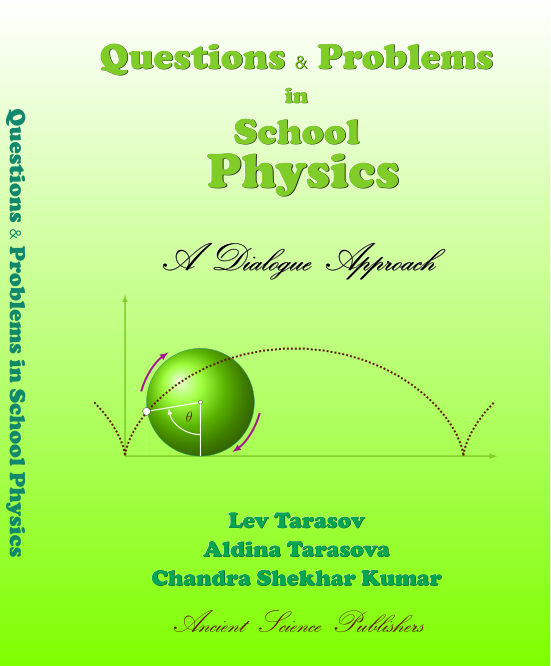
\includegraphics[width=0.5\textwidth]{tarasov-phy/cover}
  \end{center}
  %\caption{Front Cover}
\end{wrapfigure}

\section{Foreword}

\hspace{5mm}It can safely be asserted that no student preparing for an entrance examination in physics, for admission to an engineering institute has yet opened a book similar to this one. Employing the extremely lively form of dialogue, the authors were able to comprehensively discuss almost all the subjects in the syllabus, especially questions usually considered difficult to understand. The book presents a detailed analysis of common mistakes made by students taking entrance examinations in physics. Students will find this to be an exceptionally clear and interesting textbook which treats of complicated problems from various viewpoints and contains a great many excellent illustrations promoting a deeper understanding of the ideas and concepts involved. 

\vspace{2mm}

The authors are lecturers of the Moscow Institute of Electronics Engineering and are well acquainted with the general level of training of students seeking admission to engineering institutes; they have years of experience in conducting entrance examinations. The expert knowledge of the authors, in conjunction with the lively and lucid presentation, has made this a very useful study guide for students preparing for physics examinations. 


\vspace{0.2in}

 \hfill \emph{Prof. G. Epifanov, D.Sc. (Phys. and Math.)}



\section{Preface}
\thispagestyle{empty}


\hspace{5mm}This book was planned as an aid to students preparing for an entrance examination in physics for admission to an engineering institute. It has the form of a dialogue between the author (the TEACHER) and an inquisitive reader (the STUDENT). This is exceptionally convenient for analyzing common errors made by students in entrance examinations, for reviewing different methods of solving the same problems and for discussing difficult questions of physical theory. A great many questions and problems of school physics are dealt with. Besides, problems are given (with solutions) for home study. Most of the questions and problems figured in the entrance examinations of the Moscow Institute of Electronics Engineering in the years 1964-66. 

\vspace{2mm}

An analysis of mistakes made by students is always instructive. Attention can be drawn to various aspects of the problem, certain fine points can be made, and a more thorough understanding of the fundamentals can be reached. Such an analysis, however, may prove to be very difficult. Though there is only one correct answer, there can be a great many incorrect ones. It is practically impossible to foresee all the incorrect answers to any question; many of them remain concealed forever behind the distressing silence of a student being orally examined. Nevertheless, one can point out certain incorrect answers to definite questions that are heard continually. There are many questions that are almost inevitably answered incorrectly. This book is based mainly on these types of questions and problems. 

\vspace{2mm}

We wish to warn the reader that this is by no means a textbook embracing all the items of the syllabus. He will not find here a systematic account of the subject matter that may be required by the study course in physics. He will find this text to be perhaps more like a freely told story or, rather, a freely conducted discussion. Hence, it will be of little use to those who wish to begin their study of physics or to systematize their knowledge of this science. It was intended, instead, for those who wish to increase their knowledge of physics on the threshold of their examinations. 

\vspace{2mm}

Our ideal reader, as we conceive him, has completed the required course in school physics, has a good general idea of what it is all about, remembers the principal relationships, can cite various laws and has a fair knowledge of the units employed. He is in that \hlt{suspended} state in which he is no longer a secondary school student and has not yet become a full-fledged student of an institute. He is eager, however, to become one. If this requires an extension of his knowledge in physics, our book can help him. 

\vspace{2mm}

Primarily, we hope our book will prove that memorizing a textbook (even a very good one) is not only a wearisome business, but indeed a fruitless one. A student must learn to \hlt{think}, to ponder over the material and not simply learn it by heart. If such an understanding is achieved, to some extent or other, we shall consider our efforts worthwhile. 

\vspace{10mm}

\thispagestyle{empty}

In conclusion, we wish to thank Prof. G. Epifanov without whose encouragement and invaluable aid this book could not have been written and prepared for publication. We also gratefully acknowledge the many helpful suggestions and constructive criticism that were made on the manuscript by Prof. V. A. Fabrikant, Associate Prof. A. G. Chertov, and E. N. Vtorov, Senior Instructor of the Physics Department of the Moscow Power Engineering Institute. 

\vspace{0.2in}

 \hfill \hlt{Lev Tarasov}
 
  \hfill \hlt{Aldina Tarasova}

\vspace{0.2in}

Employing the extremely lively form of dialogue between the TEACHER and an inquisitive READER, this book comprehensively discusses almost all the subjects in school physics, especially questions usually considered difficult to understand.

\vspace{2mm}

In this edition, the entire manuscript was typeset using the \LaTeXe{} document processing system originally developed by \emph{Leslie Lamport}, based on \TeX{} typesetting system created by \emph{Donald Knuth}. The typesetting software used the \hologo{XeLaTeX} distribution.

\vspace{2mm}

I am grateful for this opportunity to put the materials into a consistent format, and to correct errors in the original publication that have come to my attention. The process of compiling this book has given me an incentive to improve and extend the text, dialogue, concepts, problems, solutions, layout, to double check almost all of the mathematical rendering, to correct all known errors, to improve the original illustrations by redrawing them with Till Tantau's marvellous \textup{Ti\textit{k}Z}, to include new diagrams. Thus the book now appears in a form that we hope will remain useful for at least another generation.


\vspace{3mm}

\noindent {\calligra Ancient Science Publishers}  \hfill \emph{Chandra Shekhar Kumar}


\begin{center}
AUTHOR (TEACHER)  \\
READER (STUDENT) 
\end{center}

\section{Table of Contents}

\begin{enumerate}[nosep]
  \item Can You Analyze Graphs Representing the Kinematics of Straight-Line Motion ?
  \item Can You Show The Forces Applied To A Body?
  \item Can You Determine The Friction Force?
  \item How Well Do You Know Newton’s Laws Of Motion ?
  \item How Do You Go About Solving Problems In Kinematics ?
  \item How Do You Go About Solving Problems In Dynamics ?
  \item Are Problems In Dynamics Much More Difficult To Solve If Friction Is Taken Into Account ?
  \item How Do You Deal With Motion In A Circle ?
  \item How Do You Explain The Weightlessness Of Bodies ?
  \item Can You Apply The Laws Of Conservation Of Energy And Linear Momentum ?
  \item Can You Deal With Harmonic Vibrations ?
  \item What Happens To A Pendulum In A State Of Weightlessness ?
  \item Can You Use The Force Resolution Method Efficiently ?
  \item What Do You Know About The Equilibrium Of Bodies ?
  \item How Do You Locate The Centre Of Gravity ?
  \item Do you know Archimedes’ principle ?
  \item Is Archimedes’ Principle Valid In A Spaceship ?
  \item What Do You Know About The Molecular-Kinetic Theory Of Matter ?
  \item How Do You Account For The Peculiarity In The Thermal Expansion Of Water ?
  \item How Well Do You Know The Gas Laws ?
  \item How Do You Go About Solving Problems On Gas Laws ?
  \item Let Us Discuss Field Theory
  \item How Is An Electrostatic Field Described ?
  \item How Do Lines Of Force Behave Near The Surface Of A Conductor ?
  \item How Do You Deal With Motion In A Uniform Electrostatic Field ?
  \item Can You Apply Coulomb’s Law ?
  \item Do You Know Ohm’s Law ?
  \item Can A Capacitor Be Connected Into A Direct-Current Circuit ?
  \item Can you compute the resistance of a branched portion of a circuit ?
  \item Why Did The Electric Bulb Burn Out ?
  \item Do You Know How Light Beams Are Reflected And Refracted ?
  \item How Do You Construct Images Formed By Mirrors And Lenses ?
  \item How Well Do You Solve Problems Involving Mirrors And Lenses ? 
\end{enumerate}

\hrulefill



\newtheorem{probl}{\textcolor{Gold}{\textbf{\textsc{Author}}}}[chapter]

\renewenvironment{p}    % this is the environment name for the input
  {\renewcommand{\qedsymbol}{$\lozenge$}%
   \pushQED{\qed}\begin{probl}}
  {\popQED\end{probl}}
  
\renewenvironment{s}
  {\renewcommand{\qedsymbol}{\tiny$\blacksquare$}
  \vspace{-\baselineskip}
  \begin{proof}[\emph{\textbf{\scshape \textcolor{BurntOrange}{Reader}}}]\color{zinnwalditebrown}}
  {\end{proof}} 

\underline{\textbf{\textcolor{BurntOrange}{Excerpt from the Chapter} \textcolor{Sepia}{4:}}}


\section{How Well Do You Know Newton's Laws Of Motion ?}



\begin{p}
Please state \hlt{Newton's first law of motion.}
\end{p}


\begin{s}
A body remains at rest or in a state of uniform motion in a straight line until the action of other bodies compels it to change that state. 
\end{s}


\begin{p}
Is this law valid in all frames of reference ?
\end{p}



\begin{s}
I don't understand your question. 
\end{s}


\begin{p}
If you say that a body is at rest, you mean that it is stationary with respect to some other body which, in the given case, serves as the reference system, or frame of reference. It is quite pointless to speak of a body being in a state of rest or definite motion without indicating the frame of reference. The nature of the motion of a body depends upon the choice of the frame of reference. For instance, a body lying on the floor of a traveling railway car is at rest with respect to a frame of reference attached to the car, but is moving with respect to a frame of reference attached to the track. Now we can return to my question. Is Newton's first law valid for all frames of reference ?
\end{p}


\begin{s}
Well, it probably is.
\end{s}




\begin{p}
I see that this question has taken you unawares. Experiments show that Newton's first law is not valid for all reference systems. Consider the example with the body lying on the floor of the railway car. We shall neglect the friction between the body and the floor. First we shall deal with the position of the body with respect to a frame of reference attached to the car. We can observe the following: the body rests on the floor and, all of a sudden, it begins to slide along the floor even though no action of any kind is evident. Here we have an obvious violation of Newton's first law of motion. The conventional explanation of this effect is that the car, which had been traveling in a straight line and at uniform velocity, begins to slow down, because the train is braked, and the body, due to the absence of friction, continues to maintain its state of uniform straight-line motion with respect to the railway tracks. From this we can conclude that Newton's law holds true in a frame of reference attached to the railway tracks, but not in one attached to a car being slowed down.

\hlt{Frames of reference for which Newton's first law is valid are said to be inertial; those in which it is not valid are non-inertial.} For most of the phenomena we deal with we can assume that any frame of reference is inertial if it is attached to the earth's surface, or to any other bodies which are at rest with respect to the earth's surface or travel in a straight line at uniform velocity. Non-inertial frames of reference are systems traveling with acceleration (or deceleration), for instance rotating systems, accelerating or decelerating lifts, etc. \hlt{Note that not only Newton's first law of motion is invalid for non-inertial reference systems, but his second law as well (since the first law is a particular case of the second law).}
\end{p}



\begin{s}
But if Newton's laws cannot be employed for frames of reference traveling with acceleration, then how can we deal with mechanics in such frames ?
\end{s}


\begin{p}
Newton's laws of motion can nevertheless be used for non-inertial frames of reference. To do this, however, it will be necessary to apply, purely formally, an additional force to the body. This force, the so called \hlt{inertial force}, equals the product of the mass of the body by the acceleration of the reference system, and its direction is opposite to the acceleration of the body. \hlt{I should emphasize that no such force actually exists but, if it is formally introduced, then Newton's laws of motion will hold true in a non-inertial frame of reference.}

\hlt{I want to advise you, however, to employ only inertial frames of reference in solving problems.} Then, all the forces that you have to deal with will be really existing forces.
\end{p}


\begin{s}
But if we limit ourselves to inertial frames of reference, then we cannot analyze, for instance, a problem about a body lying on a rotating disk.
\end{s}


\begin{p}
Why can't we ? The choice of the frame of reference is up to you. If in such a problem you use a reference system attached to the disk (i.e. a non-inertial system), the body is considered to be at rest. But if your reference system is attached to the earth (i.e. an inertial reference system), then the body is dealt with as one traveling in a circle.

I would advise you to choose an inertial frame of reference. And now please state \hlt{Newton's second law of motion.}
\end{p}



\begin{s}
This law can be written as \hlm{$F=ma$}, where \hlm{$F$} is the force acting on the body, \hlm{$m$} is its mass and \hlm{$a$} : acceleration.
\end{s}


\begin{p}
Your laconic answer is very typical. I should make three critical remarks on your statement; two are not very important and one is essential. In the first place, \hlt{it is not the force that results from the acceleration, but, on the contrary, the acceleration is the result of the applied force.} It is therefore more logical to write the equation of the law as
\hlm{\begin{equation}%
a=B\cdot\frac{F}{m}
\label{eq-10}
\end{equation}}
where \hlm{$B$} is the proportionality factor depending upon the choice of units of measurement of the quantities in~\cref{eq-10}. Notice that your version had no mention of the proportionality factor \hlm{$B$}. Secondly, a body is accelerated by all forces applied to it (though some may counterbalance one another). Therefore, in stating the law you should use, not the term \hlt{force}, but the more accurate term \hlt{resultant force.}

My third remark is the most important. Newton's second law establishes a relationship between force and acceleration. But force and acceleration are vector quantities, characterized not only by their numerical value (magnitude) but by their direction as well. Your statement of the law fails to specify the directions. This is an essential shortcoming. Your statement leaves out a vital part of Newton's second law of motion. Correctly stated it is: \hlt{the acceleration of a body is directly proportional to the resultant of all forces acting on the body, inversely proportional to the mass of the body and takes place in the direction of the resultant force}. This statement can be analytically expressed by the formula
\hlm{\begin{equation}%
\vec{a}=B\cdot\frac{\vec{F}}{m}
\label{eq-11}
\end{equation}}
(where the arrows over the letters denote vectors).
\end{p}




\begin{s}
When in~\cref{ch2} we discussed the forces applied to a body thrown upward at an angle to the horizontal, you said you would show later that the direction of motion of a body does not necessarily coincide with the direction of the force applied to it. You referred then to Newton's second law.
\end{s}


\begin{p}
Yes, I remember, and I think it would be quite appropriate to return to this question. Let us recall what acceleration is. As we know, acceleration is characterized by the change in velocity in unit time. Illustrated in~\cref{fig:18} are the velocity vectors \hlm{$\vv{v_{1}}$} and \hlm{$\vv{v_{2}}$} of a body for two nearby instants of time \hlm{$t$} and \hlm{$t+\Delta t$}. The change in velocity during the time \hlm{$\Delta t$} is the vector \hlm{$\Delta \vv{v} =\vv{v_{2}} - \vv{v_{1}}$}. 

\begin{figure}[H]
\centering
\begin{tikzpicture}

\draw[-latex, line width=1.7pt, xptcolor] (0,0) -- (7,0) node[above left,xptcolor] {$\vec{v_1}$};
\draw[-latex, line width=1.7pt, horzlinecolor] (7,0) -- (7,-2);
\draw (7.4,-1) node[rotate=-90,horzlinecolor] {$\vec{\Delta v}$};
\draw[-latex, line width=1.7pt, plotptcolor] (0,0) -- (7,-2);
\draw (-20:4) node[rotate=-20,plotptcolor] {$\vec{v_2}$};

\end{tikzpicture}

\caption{Change in the velocity vectors in unit time is acceleration}
\label{fig:18}
\end{figure}

By definition, the acceleration is
\hlm{\begin{equation}%
\vec{a}(t) \cong \lmts{\Delta t}{0}\frac{\Delta \vec{v}}{\Delta t}
\label{eq-12}
\end{equation}}
or, more rigorously,
\hlm{\begin{equation}%
\vec{a}(t) = \lmts{\Delta t}{0}\frac{\Delta \vec{v}}{\Delta t}
\label{eq-13}
\end{equation}}
It follows that the acceleration vector is directed along vector \hlm{$\Delta v$}, which represents the change in velocity during a sufficiently short interval of time. It is evident from~\cref{fig:18} that the velocity vectors and the change in velocity vector can be oriented in entirely different directions. This means that, \hlt{in the general case, the acceleration and velocity vectors are also differently oriented.} Is that clear ?
\end{p}



\begin{s}
Yes, now I understand. For example, when a body travels in a circle, the velocity of the body is directed along a tangent to the circle, but its acceleration is directed along a radius toward the center of rotation (I mean centripetal acceleration).
\end{s}


\begin{p}
Your example is quite appropriate. Now let us return to relationship (\cref{eq-11}) and make it clear that it is precisely the acceleration and not the velocity that is oriented in the direction of the applied force, and that it is again the acceleration and not the velocity that is related to the magnitude of this force. On the other hand, the nature of a body's motion at any given instant is determined by the direction and magnitude of its velocity at the given instant (the velocity vector is always tangent to the path of the body).

Since the acceleration and velocity are different vectors, the direction of the applied force and the direction of motion of the body may not coincide in the general case. Consequently, the nature of the motion of a body at a given instant is not uniquely determined by the forces acting on the body at the given instant.
\end{p}


\begin{s}
This is true for the general case. But, of course, the direction of the applied force and the velocity may coincide.
\end{s}



\begin{p}
Certainly, that is possible. Lift a body and release it carefully, so that no initial velocity is imparted to it. Here the direction of motion will coincide with the direction of the force of gravity. If, however, you impart a horizontal initial velocity to the body then its direction of motion will not coincide with the direction of the gravity force; the body will follow a parabolic path. Though in both cases the body moves due to the action of the same force : its weight, the nature of its motion differs. A physicist would say that this difference is due to the different initial conditions : at the beginning of the motion the body had no velocity in the first case and a definite horizontal velocity in the second.

Illustrated in~\cref{fig:19} are the trajectories of bodies thrown with initial velocities of different directions, but in all cases the same force, the weight of the body, is acting on it.
\end{p}


\begin{figure}[H]
\centering
\begin{tikzpicture}[
    declare function={f(\x)=-\x^2+ \x;}, %unit of length is cm
    declare function={g(\x)=-2*\x^2+ 1.5*\x;},
    declare function={h(\x)=-24*\x^2+ 6*\x;},  
    declare function={ft(\x)=\x;},
    declare function={gt(\x)=1.5*\x;},
    declare function={ht(\x)=6*\x;},
   % declare function={g(\x)=0.86 + .98*(\x-0.76);}, %tangent at(0.3in,0.34in) = (0.3*2.54cm, 0.34*2.54cm) is : y = 0.34*2.54cm + (2.5-2*.3*2.54cm)(x-.3*2.54cm)
    xscale=10,yscale=18
]
  %\draw[red, arrows={-Triangle[angle=45:10pt]}] (0,0.0) -- (1,0.0);
\draw[variable=\x, xptcolor, thick, samples=100, domain=0:1,smooth] plot(\x, {f(\x)});
\draw[arrows={-Triangle[angle=45:10pt]},variable=\x, xptcolor, thick, samples=100, domain=0:0.75,smooth] plot(\x, {f(\x)});  
\draw[-latex,variable=\x, xptcolor, samples=100, domain=0:0.2,smooth] plot(\x, {ft(\x)});
\draw[variable=\x, plotptcolor, thick, samples=100, domain=0:0.75,smooth] plot(\x, {g(\x)}); 
\draw[arrows={-Triangle[angle=45:10pt]},variable=\x, plotptcolor, thick, samples=100, domain=0:0.4,smooth] plot(\x, {g(\x)});  
\draw[-latex,variable=\x, plotptcolor, samples=100, domain=0:0.145,smooth] plot(\x, {gt(\x)});
\draw[variable=\x, horzlinecolor, thick, samples=100, domain=0:0.25,smooth] plot(\x, {h(\x)}); 
\draw[arrows={-Triangle[angle=45:10pt]},variable=\x, horzlinecolor, thick, samples=100, domain=0:0.19,smooth] plot(\x, {h(\x)});  
\draw[-latex,variable=\x, horzlinecolor, samples=100, domain=0:0.039,smooth] plot(\x, {ht(\x)});
%\draw[-latex,variable=\x, dotted, xptcolor, ultra thick, samples=100, domain=.255:1.5,smooth] plot(\x, {f(\x)});
%\draw[variable=\x, dotted, xptcolor, ultra thick, samples=100, domain=.255:1.245,smooth] plot(\x, {h(\x)}); 

\draw[xlabelcolor,ultra thick] (-0.1,0) -- (1.1,0);
\fill [pattern = bricks, pattern color=xlabelcolor] (-0.1,0) rectangle (1.1,-0.05);
\node[shading=ball,circle,ball color=xptcolor,inner sep=1mm] at (0.9,0.09) {};
\node[shading=ball,circle,ball color=plotptcolor,inner sep=1mm] at (0.3,0.27) {};
\node[shading=ball,circle,ball color=horzlinecolor,inner sep=1mm] at (0.15,0.36) {};
%\draw[variable=\x, -latex, ultra thick, samples=100, domain=0.76:1.2,smooth] plot(\x, {g(\x)}) node[above] {\hlm{$F$}}; 

\end{tikzpicture}

\caption{Projectiles with different initial velocities}
\label{fig:19}
\end{figure}




\begin{s}
Does that mean that the nature of the motion of a body at a given instant depends not only on the forces acting on the body at this instant, but also on the initial conditions ?
\end{s}


\begin{p}
Exactly. It should be emphasized that the initial conditions reflect the prehistory of the body. They are the result of forces that existed in the past. These forces no longer exist, but the result of their action is manifested. From the philosophical point of view, this demonstrates the relation of the past to the present, i.e, the principle of causality.

Note that if the formula of Newton's second law contained the velocity and not the acceleration, this relationship of the past and present would not be revealed. In this case, the velocity of a body at a given instant (i.e. the nature of its motion at a given instant) would be fully determined by the forces acting on the body precisely at this instant; the past would have no effect whatsoever on the present.

I want to cite one more example illustrating the aforesaid. 

A ball hanging on a string is subject to the action of two forces, the weight and the tension of the string. If it is deflected to one side of the equilibrium position and then released, it will begin to oscillate. 

\begin{figure}[H]
\centering
\begin{tikzpicture}

\fill [pattern = bricks, pattern color=Red] (-1in,0in) rectangle (1in,0.3in);
\draw[ultra thick, plotptcolor, dashed] (0,0) -- (-90:4.5cm);
\draw[ultra thick, plotptcolor] (0,0) -- (-60:4cm);
\draw[ultra thick, plotptcolor, dashed] (0,0) -- (-120:4cm);
\draw[xptcolor, ultra thick, dashed] (-120:4cm) arc(-120:-60:4cm);
\node[shading=ball,circle,ball color=Black,inner sep=2mm] (a) at (-60:4cm) {};
\node[circle,draw,ultra thick,inner sep=2.0mm] at (-120:4cm) {};
\path (a) -- ++(0,-0.6in) coordinate(P);
\draw[-latex, ultra thick, xptcolor] (a) -- (P) node[below] {$P$};
\draw[-latex, ultra thick, plotptcolor] (a) -- (-60:2cm) node[right,rotate=25] {$T_1$};;

\end{tikzpicture}

\caption{Oscillating ball}
\label{fig:20a}
\end{figure}

If, however, a definite velocity is imparted to the ball in a direction perpendicular to the plane of deviation, the ball will begin to travel in a circle at uniform velocity. 


As you can see, depending upon the initial conditions, the ball either oscillates in a plane (see~\cref{fig:20a}), or travels at uniform velocity in a circle (see~\cref{fig:20b}). Only two forces act on it in either case: its weight and the tension of the string.
\end{p}



\begin{s}
I haven't considered Newton's laws from this viewpoint.
\end{s}


\begin{p}
No wonder then that some students, in trying to determine the forces applied to a body, base their reasoning on the nature of motion without first finding out what bodies interact with the given body. You may recall that you did the same. That is exactly why, when drawing~\cref{fig:8c} and~\cref{fig:8d}, it seemed to you that the sets of forces applied to the body in those cases should be different. Actually, in both cases two forces are applied to the body: its weight and the tension of the string.
\end{p}

\begin{figure}[H]
\centering
\begin{tikzpicture}

\fill [pattern = bricks, pattern color=xlabelcolor] (-1in,0in) rectangle (1in,0.3in);
\draw[thick, xlabelcolor] (-1in,0in) -- (1in,0in);
\draw[thick, plotptcolor, dotted] (0,0) -- (-90:5cm);
\draw[ultra thick, plotptcolor] (0,0) -- (-60:4cm);
\draw[xptcolor, thick, dashed]  (2,-3.46) arc (0:180:2 and 0.7);
\draw[xptcolor, thick]  (2,-3.46) arc (0:-180:2 and 0.7);
\node[shading=ball,circle,ball color=Black,inner sep=2mm] (a) at (-60:4cm) {};
\path (a) -- ++(0,-0.6in) coordinate(P);
\draw[-latex, ultra thick, xptcolor] (a) -- (P) node[below] {$P$};
\draw[-latex, ultra thick, plotptcolor] (a) -- (-60:2cm) node[right,rotate=25] {$T_2$};;
    
\end{tikzpicture}

\caption{Motion of a ball in circle}
\label{fig:20b}
\end{figure}



\begin{s}
Now I understand that \hlt{the same set of forces can cause motions of different nature and therefore data on the nature of the motion of a body cannot serve as a starting point in determining the forces applied to the body.}
\end{s}


\begin{p}
You have stated the matter very precisely. There is no need, however, to go to the extremes. Though different kinds of motion may be caused by the same set of forces (as in~\cref{fig:20a} and~\cref{fig:20b}), the numerical relations between the acting forces differ for the different kinds of motion. This means that there will be a different resultant applied force for each motion. Thus, for instance, in uniform motion of a body in a circle, the resultant force should be the \hlt{centripetal} one; in oscillation in a plane, the resultant force should be the \hlt{restoring force}. From this it follows that even though data on the kind of motion of a body cannot serve as the basis for determining the applied forces, they are far from superfluous.

In this connection, let us return to the example illustrated in~\cref{fig:20a} and~\cref{fig:20b}. Assume that the angle \hlm{$\alpha$}, between the vertical and the direction of the string is known and so is the weight \hlm{$P$} of the body. Find the tension \hlm{$T$} in the string when 
\begin{enumerate}[label=(\arabic*)]
\item  the oscillating body is in its extreme position, and
\item when the body is traveling uniformly in a circle.
\end{enumerate}

In the first case, the resultant force is the restoring force and it is perpendicular to the string. Therefore, the weight \hlm{$P$} of the body is resolved into two components, with one component along the resultant force and the other perpendicular to it (i.e. directed along the string). Then the forces perpendicular to the resultant force, i.e. those acting in the direction along the string, are equated to each other (see~{fig:21a}). 
\hlm{\begin{equation*}%
\therefore T_{1} = P \cos \alpha
\end{equation*}}

\begin{figure}[H]
\centering
\begin{tikzpicture}

\fill [pattern = bricks, pattern color=xlabelcolor] (-1in,0in) rectangle (1in,0.3in);
\draw[thick, xlabelcolor] (-1in,0) -- (1in,0);
\draw[ultra thick, plotptcolor, dashed] (0,0) -- (-90:5cm);
\draw[ultra thick, plotptcolor] (0,0) -- (-60:4cm);
\node[circle,draw,ultra thick,inner sep=2.0mm] (a) at (-60:4cm) {};
\path (a) -- ++(0,-2.31) coordinate(P);
\path (a) -- ++(30:-1.155) coordinate(P1);
\draw[-latex, ultra thick, xptcolor] (-60:4) -- (P) node[below] {$P$};
\draw[-latex, ultra thick, plotptcolor] (-60:4) -- (P1);
\draw[-latex, ultra thick, plotptcolor] (a) -- (-60:2cm) node[right,rotate=30] {$T_1$};;
%\draw[xptcolor, thick]  (0,-1) arc (270:300:1);
%\draw[xptcolor, thick]  (0,-1.1) arc (270:300:1.1);
%\draw[xptcolor, thick]  (0.4,-1.3) node[rotate=30] {$\alpha$};
\tkzDefPoint(0,-1){l}
\tkzDefPoint(0,0){O}
\tkzDefPoint(-60:1){m}
\tkzMarkAngle[size = 1.0,arc=ll,color=xptcolor](l,O,m)
\tkzLabelAngle[pos=1.3,rotate=30,color=xptcolor](l,O,m) {$\alpha$}
\path (a) -- ++(-150:2) coordinate(Q);
\path (a) -- ++(30:1) coordinate(R);
\draw[horzlinecolor,dashed] (Q) -- (R);
\draw[-latex, ultra thick, horzlinecolor] (-60:4) -- (-60:6) coordinate(b) node[right,rotate=30] {$P\cos\alpha$};
\tkzMarkAngle[size = 1.0,arc=ll,color=xptcolor](P,a,b)
\tkzLabelAngle[pos=1.3,rotate=30,color=xptcolor](P,a,b) {$\alpha$}
\tkzDefPoint(-60:2){u}
\tkzMarkSegments[mark=||](a,u a,b)
\draw[ultra thick, horzlinecolor,dotted] (P) -- (P1) (P) -- (b);
%\draw[-latex, ultra thick, horzlinecolor] (a) -- (P1);
%\tkzDrawLine[altitude](P,Q,R)
%\tkzDefLine[perpendicular=through P,K=-1](Q,R) \tkzGetPoint{p}
%\draw[-latex, ultra thick, plotptcolor] (a) -- (p);
\end{tikzpicture}

\caption{Forces on the oscillating ball}
\label{fig:21a}
\end{figure}

In the second case, the resultant force is the centripetal one and is directed horizontally. Hence, the tension \hlm{$T_{2}$} of the string should be resolved into a vertical and a horizontal force, and the forces perpendicular to the resultant force, i.e, the vertical forces, should be equated to each other (\cref{fig:21b}). 

\hlm{\begin{equation*}%
\therefore T_{2} \cos \alpha = P \quad \text{or} \quad T_{2} = \frac{P}{\cos \alpha}
\end{equation*}}


\begin{figure}[H]
\centering
\begin{tikzpicture}

\fill [pattern = bricks, pattern color=xlabelcolor] (-1in,0in) rectangle (1in,0.3in);
\draw[thick, xlabelcolor] (-1in,0) -- (1in,0);
\draw[ultra thick, plotptcolor, dashed] (0,0) -- (-90:5cm) coordinate(y);
\draw[ultra thick, plotptcolor] (0,0) -- (-60:4cm);
\node[circle,draw,ultra thick,inner sep=2.0mm] (a) at (-60:4cm) {};
\path (a) -- ++(0,-1.73) coordinate(P);
\path (a) -- ++(0,1.73) coordinate(P1);
%\path (a) -- ++(30:-1.155) coordinate(P1);
\draw[-latex, ultra thick, xptcolor] (-60:4) -- (P) node[below] {$P$};
\draw[-latex, ultra thick, plotptcolor] (-60:4) -- (P1) node[right] {$T_2 \cos\alpha$};
\draw[-latex, ultra thick, plotptcolor] (a) -- (-60:2cm) node[left,rotate=30] {$T_2$};;

\tkzDefPoint(0,-1){l}
\tkzDefPoint(0,0){O}
\tkzDefPoint(-60:1){m}
\tkzDefPoint(-60:2){n}
\tkzMarkAngle[size = 0.7,arc=ll,color=xptcolor](l,O,m)
\tkzLabelAngle[pos=0.9,rotate=30,color=xptcolor](l,O,m) {$\alpha$}
\tkzMarkAngle[size = 0.7,arc=ll,color=xptcolor](P1,a,n)
\tkzLabelAngle[pos=0.9,rotate=30,color=xptcolor](P1,a,n) {$\alpha$}
%\path (a) -- ++(-150:2) coordinate(Q);
%\path (a) -- ++(30:1) coordinate(R);
%\draw[horzlinecolor,dashed] (Q) -- (R);
%\draw[-latex, ultra thick, horzlinecolor] (-60:4) -- (-60:6) coordinate(b) node[right,rotate=30] {$P\cos\alpha$};
%\tkzMarkAngle[size = 1.0cm,arc=ll,color=xptcolor](P,a,b)
%\tkzLabelAngle[pos=1.3,rotate=30,color=xptcolor](P,a,b) {$\alpha$}
\tkzMarkSegments[mark=||](a,P a,P1)
%\draw[ultra thick, horzlinecolor,dotted] (P) -- (P1) (P) -- (b);
\draw[thick, horzlinecolor, dashed, shorten >= 0.3cm, shorten <= -0.8cm] (-60:4) -- ($(O)!(a)!(y)$); % $(O)!(a)!(y)$ is a projection of the point a on the line Oy
\draw[ultra thick, horzlinecolor, dotted] (n) -- ($(a)!(n)!(P1)$);
\draw[ultra thick, horzlinecolor, dotted] (n) -- ($(a)!(n)!($(O)!(a)!(y)$)$);
\draw[-latex, ultra thick, horzlinecolor] (a) -- ($(a)!(n)!($(O)!(a)!(y)$)$);
%\draw[-latex, ultra thick, horzlinecolor] (a) -- (P1);
%\tkzDrawLine[altitude](P,Q,R)
%\tkzDefLine[perpendicular=through P,K=-1](Q,R) \tkzGetPoint{p}
%\draw[-latex, ultra thick, plotptcolor] (a) -- (p);
\end{tikzpicture}

\caption{Forces on the moving ball in circle}
\label{fig:21b}
\end{figure}

As you can see, a knowledge of the nature of the body's motion proved useful in finding the tension of the string.
\end{p}


\begin{s}
If I understand all this correctly, then, knowing the interaction of bodies, you can find the forces applied to one of them; if you know these forces and the initial conditions, you can predict the nature of the motion of the body (the magnitude and direction of its velocity at any instant).

On the other hand, if you know the kind of motion of a body you can establish the relationships between the forces applied to it. Am I reasoning correctly?
\end{s}



\begin{p}
Quite so. But let us continue. I want to propose a comparatively simple problem relating to Newton's second law of motion. 

\hlt{Two bodies, of masses \hlm{$M$} and \hlm{$m$}, are raised to the same height above the floor and are released simultaneously. Will the two bodies reach the floor simultaneously if the resistance of the air is the same for each of them? For simplicity we shall assume that the air resistance is constant.}
\end{p}

\begin{s}
Since the air resistance is the same for the two bodies, it can be disregarded. Consequently, both bodies reach the floor simultaneously.
\end{s}


\begin{p}
You are mistaken. You have no right to disregard the resistance of the air. Take, for example, the body of mass \hlm{$M$}. It is subject to two forces: the weight \hlm{$Mg$} and the air resistance \hlm{$F$}. The resultant force is \hlm{$Mg - F$}. From this we find the acceleration. Thus
\hlm{\begin{equation*}%
a = \dfrac{Mg - F}{M} = g - \dfrac{F}{M}
\end{equation*}}
In this manner, the body of larger mass has a higher acceleration and will, consequently, reach the floor first.

Once more I want to emphasize that in calculating the acceleration of a body it is necessary to take into account all the forces applied to it, i.e. you must find the resultant force. In this connection, the use of the term \hlt{driving force} is open to criticism. This term is inappropriate. In applying it to some force (or to several forces) we seem to single out the role of this force (or forces) in imparting acceleration to the body. As if the other forces concerned were less essential. This is absolutely wrong. \hlt{The motion of a body is a result of the action of all the forces applied to it without any exceptions (of course, the initial conditions should be taken into account).}

Let us now consider an example on \hlt{Newton’s third law of motion}. A horse starts to pull a wagon. As a result, the horse and wagon begin to travel with a certain acceleration. 

\begin{figure}[H]
\centering
\begin{tikzpicture}[y=0.80pt, x=0.80pt, scale=-0.5]%yscale=-0.2, xscale=-0.2]%, inner sep=0pt, outer sep=0pt,
even odd rule]

\fill [pattern = bricks, pattern color=xlabelcolor] (3in,3.5in) rectangle (-6in,2.0in);
%\begin{scope}[shift={(-891.18847,366.43251)}]
      %\begin{scope}[cm={{-2.67454,0.0,0.0,2.67403,(1596.5431,-564.7219)}},draw,line width=0.526pt,miter limit=4.00]
      % front first leg
        \path[draw,ball color=horsecolor,even odd rule,line cap=butt,line join=miter,line width=0.526pt,miter limit=4.00] (201.7321,169.0993) .. controls (210.6547,168.5150) and (222.6633,176.8008) .. (234.1592,184.7189) .. controls (240.7621,186.7291) and (252.0399,193.5261) .. (249.7262,200.2990) .. controls (246.7657,208.9652) and (246.6050,221.8705) .. (246.4940,231.9747) .. controls (245.8476,237.1462) and (243.2618,238.4391) .. (241.9689,240.3785) .. controls (240.6760,242.3178) and (240.6760,244.9035) .. (239.3831,246.8429) .. controls (238.0903,248.7822) and (235.5045,250.0751) .. (232.9187,252.0144) .. controls (230.3330,253.9537) and (227.7472,256.5395) .. (225.8079,257.1859) .. controls (223.8685,257.8324) and (222.5756,256.5395) .. (222.5756,254.6002) .. controls (224.1107,250.5565) and (223.6015,244.8050) .. (226.2211,241.4175) .. controls (227.5140,240.7710) and (230.3330,241.0249) .. (232.9187,239.7320) .. controls (235.5045,238.4391) and (238.0903,233.2676) .. (238.0903,230.6818) .. controls (238.0903,228.0961) and (235.5045,228.0961) .. (234.2116,227.4496) .. controls (232.9187,226.8032) and (232.9187,225.5103) .. (233.5652,224.2174) .. controls (234.2116,222.9245) and (235.5045,221.6316) .. (236.7974,219.0459) .. controls (239.7857,213.2305) and (240.2647,207.2146) .. (236.7974,201.5919) .. controls (233.1465,196.1300) and (225.7875,197.0510) .. (219.9899,196.4204) .. controls (214.8183,195.7740) and (199.7797,194.4811) .. (193.6451,189.5606);


   % back first leg
        \path[draw,ball color=horsecolor,even odd rule,line cap=butt,line join=miter,line width=0.526pt,miter limit=4.00] (116.8889,186.5926) .. controls (125.4438,210.0510) and (112.2568,211.5131) .. (106.2161,220.9852) .. controls (103.1212,230.3523) and (109.8691,239.0367) .. (115.9127,245.5500) .. controls (119.7835,249.4235) and (124.9663,251.3812) .. (128.1951,255.8931) .. controls (132.2799,261.4739) and (132.0738,268.0905) .. (132.0738,274.6399) .. controls (130.7083,279.8349) and (121.6600,270.2560) .. (119.7914,268.1755) .. controls (117.8521,265.5897) and (119.1449,264.2968) .. (119.1449,262.3575) .. controls (119.1449,260.4181) and (117.8521,257.8324) .. (116.5592,257.1859) .. controls (115.2663,256.5395) and (113.9734,257.8324) .. (112.6805,257.8324) .. controls (111.3876,257.8324) and (110.0948,256.5395) .. (109.4483,254.6002) .. controls (108.8471,248.6065) and (106.9058,245.5539) .. (102.3374,241.6713) .. controls (98.4588,238.4391) and (91.9944,233.2676) .. (88.7622,229.3889) .. controls (85.5300,225.5103) and (85.5300,222.9245) .. (86.8228,221.6316) .. controls (90.9452,219.2854) and (92.7218,218.3762) .. (93.2376,212.4710) .. controls (93.2376,209.2388) and (89.3037,195.8939) .. (88.0108,190.7224);


  % body, back second leg, tail
        \path[draw,ball color=horsecolor,even odd rule,line cap=butt,line join=miter,line width=0.526pt,miter limit=4.00] (232.9187,115.6151) .. controls (219.7563,131.8228) and (221.7872,150.8868) .. (219.9899,170.5131) .. controls (218.6970,181.5026) and (216.1112,187.9670) .. (210.9397,192.4921) .. controls (205.7681,197.0172) and (198.0108,199.6030) .. (187.6678,201.5423) .. controls (159.0377,208.0009) and (139.7049,206.9899) .. (113.3269,198.3597) .. controls (108.8019,197.0668) and (104.9232,197.0668) .. (101.6910,199.0062) .. controls (92.8122,215.0779) and (89.7743,217.5692) .. (73.9548,220.7420) .. controls (70.7226,222.6813) and (68.1368,226.5600) .. (66.1975,233.0244) .. controls (64.2582,239.4888) and (62.9653,248.5390) .. (64.9046,254.3570) .. controls (66.8439,260.1749) and (72.0155,262.7607) .. (75.8941,266.6394) .. controls (79.7728,270.5180) and (82.3585,275.6896) .. (82.3585,278.2753) .. controls (80.0244,282.0729) and (70.6392,280.2070) .. (68.0760,279.5682) .. controls (66.1367,278.2753) and (66.1367,275.6896) .. (65.4902,273.1038) .. controls (64.8438,270.5180) and (63.5509,267.9322) .. (61.6116,267.2858) .. controls (59.6723,266.6394) and (57.0865,267.9322) .. (55.7936,265.9929) .. controls (54.5007,264.0536) and (54.5007,258.8821) .. (55.1472,254.3570) .. controls (58.9721,242.6745) and (53.7032,231.1402) .. (53.8543,219.4491) .. controls (54.5007,214.9240) and (58.3794,214.9240) .. (60.9652,213.6311) .. controls (66.2590,210.5104) and (66.2379,205.3094) .. (64.8438,200.0558) .. controls (63.5509,195.5307) and (60.9652,185.4309) .. (59.6723,179.6129) .. controls (58.3794,173.7949) and (58.3794,169.9163) .. (59.0258,166.6841) .. controls (59.6723,163.4519) and (60.9651,160.8661) .. (60.9651,159.5732) .. controls (47.8166,156.5745) and (42.6944,164.7989) .. (42.5611,173.2949) .. controls (42.4903,177.8083) and (48.6359,190.7640) .. (43.4238,202.9700) .. controls (41.0005,207.5082) and (36.1900,211.3528) .. (27.3502,213.8743) .. controls (46.0283,196.6756) and (26.2323,177.1985) .. (24.7644,163.4519) .. controls (24.7795,158.6425) and (26.6909,154.9610) .. (29.6880,152.2885) .. controls (40.9846,143.2477) and (54.6328,140.2214) .. (63.5509,154.4017) .. controls (78.9782,132.0680) and (101.3646,141.7435) .. (126.2558,142.7657) .. controls (139.8311,142.7657) and (151.4670,142.7657) .. (158.5779,142.1193) .. controls (172.2007,141.5393) and (174.2605,126.3465) .. (180.4051,116.6195) .. controls (193.7433,95.5049) and (215.6713,81.5666) .. (241.1707,84.2974);



        \path[draw,ball color=horsecolor,even odd rule,line cap=butt,line join=miter,line width=0.526pt,miter limit=4.00] (78.1198,268.7859) .. controls (73.1120,268.4697) and (69.0991,268.7677) .. (65.3775,272.2253);



        \path[draw,ball color=horsecolor,even odd rule,line cap=butt,line join=miter,line width=0.526pt,miter limit=4.00] (252.3341,95.5893) .. controls (252.3341,91.4962) and (252.3341,87.4031) .. (251.0414,83.3100) .. controls (250.1965,80.6349) and (248.7994,77.9597) .. (247.5719,76.2369) .. controls (246.1916,74.5194) and (245.1852,73.4908) .. (244.6645,76.2618) .. controls (243.0874,81.7037) and (244.5777,86.4195) .. (244.5777,91.4962);



        \path[draw,ball color=horsecolor,even odd rule,line cap=butt,line join=miter,line width=0.526pt,miter limit=4.00] (205.1873,189.4820) .. controls (202.4560,204.8378) and (205.3512,209.2042) .. (204.4753,215.1672) .. controls (203.4816,221.9318) and (204.0766,228.6004) .. (203.2432,235.2069) .. controls (202.8312,238.4730) and (200.0110,241.0249) .. (198.7181,245.5500) .. controls (197.4252,250.0751) and (197.4252,256.5395) .. (198.0717,260.4182) .. controls (197.5956,268.5050) and (205.3511,266.8094) .. (208.4755,272.7006) .. controls (211.0613,275.9328) and (213.6471,281.1043) .. (214.2935,284.3365) .. controls (214.9399,287.5687) and (213.6471,288.8616) .. (209.7684,288.8616) .. controls (205.8898,288.8616) and (200.5966,287.5687) .. (198.6573,284.9830) .. controls (196.7180,282.3972) and (199.3037,278.5185) .. (199.3037,276.5792) .. controls (197.4375,272.6147) and (192.7262,274.6658) .. (190.2535,273.9934) .. controls (188.9607,273.3470) and (187.6678,272.0541) .. (187.6678,270.1148) .. controls (187.6678,268.1755) and (188.9607,265.5897) .. (188.9607,261.7110) .. controls (188.9607,257.8324) and (187.6678,252.6609) .. (187.6678,246.1964) .. controls (187.6678,239.7320) and (188.9607,231.9747) .. (188.3142,222.9245) .. controls (187.6678,213.8743) and (180.7949,196.6059) .. (178.2091,186.2629);


% face
        \path[draw,ball color=horsecolor,even odd rule,line cap=butt,line join=miter,line width=0.526pt,miter limit=4.00] (240.6760,84.5859) .. controls (241.9689,84.5859) and (243.2618,84.5859) .. (245.2011,84.5859) .. controls (247.1404,84.5859) and (249.7262,84.5859) .. (251.6655,85.8788) .. controls (253.6049,87.1717) and (254.8978,89.7575) .. (256.1906,94.2826) .. controls (257.4835,98.8077) and (259.8756,105.3854) .. (258.7764,111.7365) .. controls (257.1712,121.0114) and (260.9694,130.6092) .. (258.7764,137.5942) .. controls (258.3895,138.8264) and (257.9208,138.9004) .. (258.0030,140.9430) .. controls (258.0959,143.2520) and (257.8591,147.4786) .. (254.8978,148.5837) .. controls (248.7424,151.7676) and (246.7122,146.7258) .. (244.5547,140.8264) .. controls (243.1452,136.9050) and (241.2694,138.0709) .. (242.9017,140.8264) .. controls (244.2039,144.3644) and (246.4080,153.4366) .. (240.6760,149.2301) .. controls (239.3832,147.9373) and (238.0903,145.3515) .. (237.4438,142.7657) .. controls (236.7974,140.1799) and (236.7974,137.5942) .. (236.1509,135.0084) .. controls (234.9120,126.1872) and (225.8838,128.5817) .. (225.1614,119.4938);



        \path[draw,ball color=horsecolor,even odd rule,line cap=butt,line join=miter,line width=0.526pt,miter limit=4.00] (247.7565,91.7423) .. controls (247.4178,91.0276) and (247.7786,90.0667) .. (247.4285,89.3642) .. controls (246.4416,87.3848) and (245.3625,85.5027) .. (243.9314,83.9922) .. controls (240.8264,82.1090) and (238.5325,79.9741) .. (236.1889,77.1340) .. controls (233.9515,74.1895) and (233.2206,72.9003) .. (233.3082,77.4936) .. controls (233.4466,80.9472) and (234.3955,85.7658) .. (236.8213,89.4497) .. controls (238.1141,91.4962) and (241.0389,91.7423) .. (242.3317,91.7423);


% head hair
        \path[draw,ball color=horsecolor,even odd rule,line cap=butt,line join=miter,line width=0.526pt,miter limit=4.00] (253.7331,91.8654) .. controls (261.3090,92.6446) and (265.0930,98.9449) .. (262.6760,107.1865) .. controls (261.3833,110.5974) and (260.1968,111.2344) .. (257.5051,111.9617) .. controls (256.9118,108.2596) and (256.1850,107.9313) .. (255.5660,104.4577) .. controls (255.0362,106.4824) and (254.2098,107.0073) .. (252.9805,108.5508) .. controls (252.4507,106.7722) and (252.3341,106.5043) .. (251.6878,103.7755) .. controls (250.2900,94.1050) and (246.7242,93.9269) .. (241.5726,96.7237) .. controls (239.7256,97.7265) and (238.7648,99.2401) .. (235.1582,97.9599);



        \path[draw,ball color=horsecolor,even odd rule,line cap=butt,line join=miter,line width=0.526pt,miter limit=4.00] (245.6881,115.6642) .. controls (246.3797,113.7256) and (250.3479,112.9963) .. (250.1796,115.4181) .. controls (250.4206,117.7259) and (246.4524,117.2248) .. (245.6881,115.6642) -- cycle;



        \path[draw,ball color=horsecolor,even odd rule,line cap=butt,line join=miter,line width=0.526pt,miter limit=4.00] (249.2369,146.7816) .. controls (250.9139,144.7083) and (253.7372,144.6477) .. (254.2198,147.1507) .. controls (254.2198,148.2558) and (252.3578,150.2591) .. (251.7866,150.2591) .. controls (251.2155,150.2591) and (249.2369,147.8867) .. (249.2369,146.7816) -- cycle;



        \path[draw,ball color=horsecolor,even odd rule,line cap=butt,line join=miter,line width=0.526pt,miter limit=4.00] (252.3341,116.0548) .. controls (252.1866,113.3290) and (250.7428,112.1237) .. (249.1060,112.1385) .. controls (245.8772,112.1678) and (244.9628,114.2783) .. (242.7135,114.5932);



        \path[draw,ball color=horsecolor,even odd rule,line cap=butt,line join=miter,line width=0.526pt,miter limit=4.00] (232.9187,239.7320) .. controls (234.2116,241.0249) and (235.5045,242.3178) .. (235.5045,244.2571) .. controls (235.5045,246.1964) and (233.9784,249.4818) .. (232.6855,252.0675);



        \path[draw,ball color=horsecolor,even odd rule,line cap=butt,line join=miter,line width=0.526pt,miter limit=4.00] (210.9645,276.2504) .. controls (206.9848,276.2434) and (202.2076,276.9384) .. (198.7429,278.6649);



        \path[cm={{-0.26086,0.0,0.0,0.27531,(263.793,24.0347)}},draw,fill=black,line width=1.961pt,miter limit=4.00] (59.6113,337.0374)arc(-250.249:109.653:3.571429 and 5.159);

    \draw[ultra thick, rounded corners, shading=ball, ball color=plotptcolor] (190,185) rectangle ++(-400,10);          
    \node[ultra thick,circle,draw,fill=Snow,inner sep=4] (a) at (190,185) {};
    \node[shading=ball,circle,ball color=plotptcolor,inner sep=2] at (a) {};
    \draw[-latex, line width=1.7pt, horzlinecolor] (140,170) -- (290,170) node[left,horzlinecolor] {$F$};
    \draw[-latex, line width=1.7pt, ballpoint] (140,170) -- (100,170) node[right,ballpoint] {$f_0$};
    \node[shading=ball,circle,ball color=ballpoint,inner sep=2.5] at (140,170) {};

\begin{scope}[shift={(-500,120)}]
    \draw[ultra thick, rounded corners, shading=ball, ball color=plotptcolor] (0,0) rectangle (300,100);  
    \node[ultra thick,circle,draw,fill=Snow,inner sep=10] at (200,100) {};
    \node[shading=ball,circle,ball color=plotptcolor,inner sep=4] at (200,100) {};
    \node[ultra thick,circle,draw,fill=Snow,inner sep=10] at (100,100) {};
    \node[shading=ball,circle,ball color=plotptcolor,inner sep=4] at (100,100) {};

    \draw[-latex, line width=1.7pt, ballpoint] (150,50) -- (190,50) node[left] {$f_0$};
    \draw[-latex, line width=1.7pt, ballpoint] (150,50) -- (50,50) node[right] {$f$};
    \node[shading=ball,circle,ball color=Black,inner sep=2.5] at (150,50) {};
   
    \draw[-latex, line width=1.7pt, horzlinecolor] (150,220) -- (250,220) node[left,horzlinecolor] {$f$};
    \draw[-latex, line width=1.7pt, horzlinecolor] (150,220) -- (0,220) node[right,horzlinecolor] {$F$};
    \node[shading=ball,circle,ball color=Black,inner sep=2.5] at (150,220) {};
\end{scope}
     % \end{scope}
%\end{scope}

\end{tikzpicture}

\caption{Horse Pulling a Wagon}
\label{fig:22}
\end{figure}

According to Newton’s third law, whatever the force with which the horse pulls the wagon, the wagon pulls back on the horse with exactly the same force but in the opposite direction. This being so, \hlt{why do the horse and wagon travel forward with an acceleration ? Please explain.}
\end{p}




\begin{s}
I have never given this any thought but I see no contradictions. The acceleration would be difficult to explain if the force with which the horse acts on the wagon was counterbalanced by the force with which the wagon acts on the horse. But these forces cannot cancel each other since they are applied to different bodies: one to the horse and the other to the wagon.
\end{s}


\begin{p}
Your explanation is applicable to the case when the wagon is not harnessed to the horse. Then the horse pushes away from the wagon, as a result of which the wagon moves in one direction and the horse in the other. The case I proposed is entirely different. The horse is harnessed to the wagon. Thus they are linked together and travel as a single system. The forces of interaction between the horse and wagon that you mentioned are applied to different parts of the same system. In the motion of this system as a whole, these forces can be regarded as mutually counterbalancing forces. Thus, you haven't yet answered my question.
\end{p}



\begin{s}
Well, then I can't understand what the matter is. Maybe the action here is not fully counterbalanced by the reaction ? After all a horse is a living organism.
\end{s}


\begin{p}
Now don't let your imagination run away with you. It was sufficient for you to meet with some difficulty and you are ready to sacrifice one of the principal laws of mechanics. To answer my question, there is no need to revise Newton's third law of motion. On the contrary, let us use this law as a basis for our discussion.

According to the third law. the interaction of the horse and the wagon cannot lead to the motion of this system as a whole (or, more precisely, it cannot impart acceleration to the system as a whole). This being so, there must exist some kind of supplementary interaction. In other words at least one more body must participate in the problem in addition to the horse and wagon. This body, in the given case is the earth. As a result, we have three interactions to deal with instead of one, namely: 
\begin{enumerate}[label=(\arabic*),leftmargin=1cm]
\item between the horse and the wagon (we shall denote this force by \hlm{$f_{0}$}; 
\item between the horse and the earth (force \hlm{$F$}), in which the horse pushes against the ground; and 
\item between the wagon and the earth (force \hlm{$f$}) which is the friction of the wagon against the ground.
\end{enumerate}

All bodies are shown in~\cref{fig:22} : the horse, the wagon and the earth and two forces are applied to each body. These two forces are the result of the interaction of the given body with the two others. The acceleration of the horse-wagon system is caused by the resultant of all the forces applied to it. There are \hlt{four} such forces and their resultant is \hlm{$F - f$}. This is what causes the acceleration of the system. Now you see that this acceleration is not associated with the interaction between the horse and the wagon.
\end{p}



\begin{s}
So the earth's surface turns out to be, not simply the place on which certain events occur, but an active participant of these events.
\end{s}


\begin{p}
Your pictorial comment is quite true. Incidentally, if you locate the horse and wagon on an ideal icy surface, thereby excluding all horizontal interaction between this system and the earth, there will be no motion, whatsoever. It should be stressed that no internal interaction can impart acceleration to a system as a whole. This can be done only by external action (you can't lift yourself by your hair, or bootstraps either). This is an important practical inference of Newton's third law of motion.
\end{p}

\hrulefill

\foreach \x in {1,...,11}
{
\includegraphics[width=2.0\linewidth]{tarasov-phy/ch4-p\x}
}








